\section{White box lumped model: RC network}
\subsection{White box lumped model}

The objective of the house model for this project is to serve as test environment for a heat pump model, what means that the house model is intended as a tool to help taking building systems design decisions. The house heating needs calculation model implemented for this project is a white box lumped model. Specifically, it is a RC network model consisting of resistances (R) and capacities (C). The RC network model is based on electrical systems analogy. The simulation of thermodynamic systems characterizing building elements as resistances or capacities allows to simplify the model while maintaining a high simulation results accuracy (Bagheri et al., Bacher et al.).  
There are several types of RC models, the most common being 3R4C models and 3R2C models which are applied on the outer and internal wall. For the simulation of simple house buildings 3R2C models perform as accurate as more complex 3R4C models (Fraisse et al. ). Considering that one of the objectives for this project is to obtain a fast but accurate simulation of a simple dwelling the 3R2C network model appeared as starting point. In the 3R2C model two indoor temperature nodes in the dwelling with capacities (usually an air and a wall temperature) and a well-known outdoor temperature are present. Between these 3 temperature nodes 3 heat transfer resistances are present. However, the direct heat transfer between the inner walls and the outdoor air is low. Moreover, uncertainties are present about heat transfer coefficients between walls and indoor air, different indoor temperatures in the house rooms and the ground temperature which deviates from the outdoor temperature. In addition, occupancy behaviour varies strongly. For that reason, we have made a further simplification to a 2R2C model. In section 4 it is shown that this dwelling model delivers a reliable annual energy consumption.


\subsection{House Model R and C Values}

This section presents the basic information for calculating a house model based on an RC network. This category of house models, analogous to electrical impedance networks, may have different numbers of R and C components, and may have various component topology. For the specific model properties, references will be given.

In heat transfer theory the basic thermal circuit contains thermal resistances. Heat transfer occurs via conduction, convection and radiation. In analogy with Ohm's Law for electricity, expressions can be derived for the heat transfer rate (analogous to electrical current) and the thermal resistances (analogous to ohmic resistances) in these three modes of heat transfer. The temperature difference plays a role analogous to the electrical voltage difference. These expressions are shown in Fig.\ref{table_1}.
\begin{figure}[H]
	\centering
	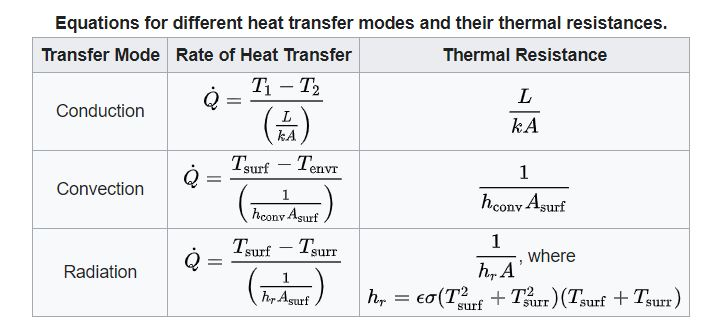
\includegraphics[width=0.8\columnwidth]{Pictures/heat transfer mode.JPG}
	\caption[Short title]{Heat transfer modes\cite{GIGO}}
	\label{table_1}
\end{figure}
\newpage

In \cite{HTTHERMO} and \cite{FUND} the expressions in Fig.\ref{table_1} are derived.
For conduction, the expression for an absolute thermal resistance:  $R = \frac{L}{kA}$ [$\frac{K}{W}$].

\begin{itemize}
    \item $L$ is the distance over which heat transfer takes place, or the thickness of the material $[m]$.
    \item $k$ is the thermal conductivity  [$\frac{W}{mK}$].
    \item $A$ is the conductive surface area  $[m^2]$.
    \item Thermal resistivity is the reciprocal of thermal conductivity and can be expressed as $r =\frac{1}{k}$ $[\frac{mK}{W}]$

\end{itemize}


For convection, and radiation the thermal resistance: $R = \frac{1}{h \cdot A}$ [$\frac{K}{W}$].

\begin{itemize}
    \item $A$ is the surface area where the heat transfer takes place $[m^2]$.
    \item $h$  heat transfer coefficient  [$\frac{W}{m^2K}$]
\end{itemize}

R\textsubscript{c}-values or RSI-values (insulation) is the building industry term for thermal resistance per unit area \cite{Rvalues_insulation} [$\frac{m^2K}{W}$].

Some typical heat transfer thermal resistance values are: \cite{OVERALL}: 

\begin{itemize}
	\item Static layer of air, 40 mm thickness (1.57 in)  : R = 0.18 [$\frac{m^2K}{W}$].
	\item Inside heat transfer resistance, horizontal current : R = 0.13 [$\frac{m^2K}{W}$]. 
	\item Outside heat transfer resistance, horizontal current : R = 0.04 [$\frac{m^2K}{W}$].
	\item Inside heat transfer resistance, heat current from down upwards : R = 0.10 [$\frac{m^2K}{W}$].
	\item Outside heat transfer resistance, heat current from above downwards : R = 0.17 [$\frac{m^2K}{W}$].
	
\end{itemize}

\begin{figure}[H]
	\centering
	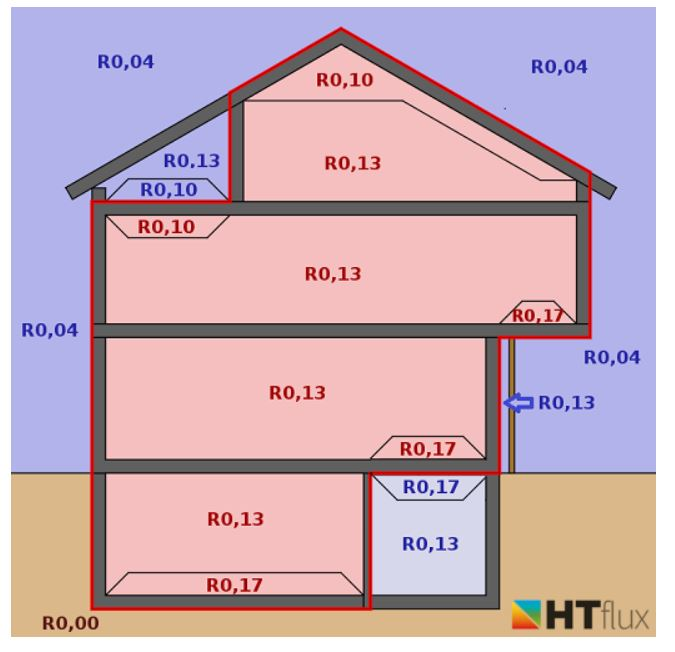
\includegraphics[width=0.8\columnwidth]{Pictures/Overview of heat resistances.JPG}
	\caption[Short title]{An overview of heat transfer resistance\cite{SURFREST}}
	\label{fig:overview}
\end{figure}


The standard R\textsubscript{c}-values that have been used for facades, roof and floor until 2020 are summarized in Fig.\ref{fig:Rcvalues}:

\begin{figure}[H]
	\centering
	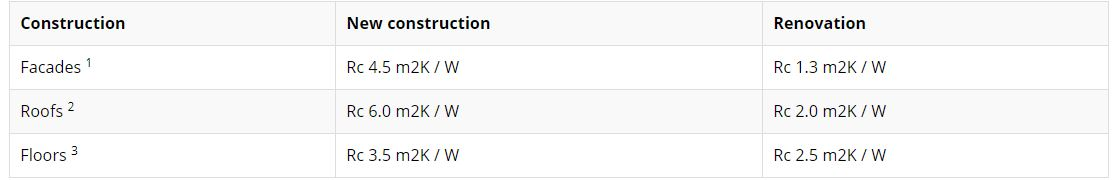
\includegraphics[width=1.0\columnwidth]{Pictures/Rc_values_2020.JPG}
	\caption[Short title]{Rc Values \cite{ISOL}}
	\label{fig:Rcvalues}
\end{figure}

New standard values will be used from 1-1-2021, since the building standard NEN 1068 will be replaced by the NTA 8800 standard. The old and new situation is described in "EnergieVademecum Energiebewust ontwerpen van nieuwbouwwoningen", chapter 5: Thermische isolatie, thermische bruggen en luchtdichtheid.
\cite{ISSO}.

\begin{figure}[H]
	\centering
	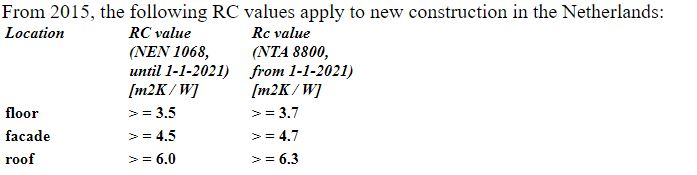
\includegraphics[width=1.0\columnwidth]{Pictures/Rc_values_2021.JPG}
	\caption[Short title]{Rc Values \cite{RVALUE}}
	\label{fig:newRc}
\end{figure}

The values used for different types of houses such as: row houses, detached houses and apartments can be found in the document "Voorbeeldwoningen 2011" \cite{VOORBEELD}. An example with values for a common type of row house, built in the period from 1975 to 1991 is shown in Fig.\ref{row_house}:


\begin{figure}[H]
	\centering
	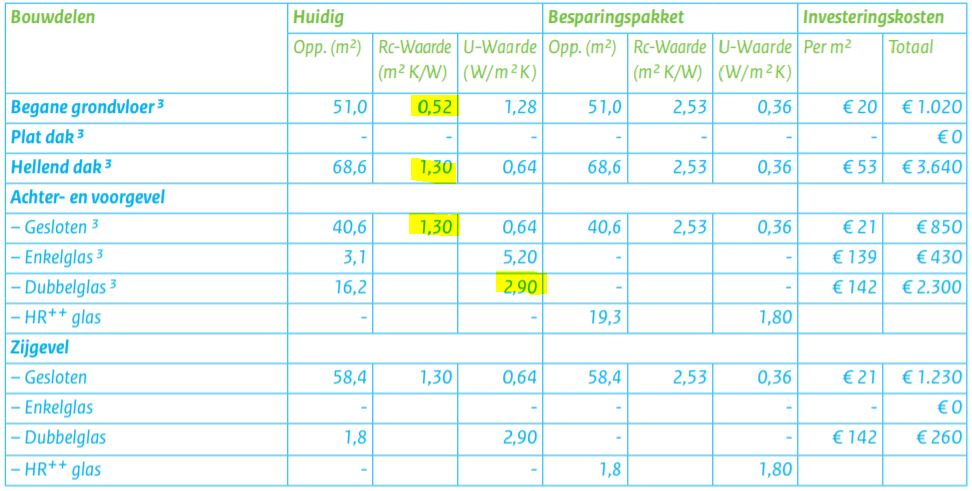
\includegraphics[width=0.8\columnwidth]{Pictures/row_house_1975-1991.JPG}
	\caption[Short title]{R\textsubscript{c}-values for a row house type built between 1975-1991 \href{Voorbeeldwoningen 2011 bestaande bouw.pdf}{[7].}}
	\label{row_house}
\end{figure} 
\newpage

\subsection{Dwelling (envelope) model analogous to a 2R-2C network}

The heat flow will be modelled by analogy to an electrical circuit where heat flow is represented by current, temperatures are represented by voltages, heat sources are represented by constant current sources, absolute thermal resistances are represented by resistors and thermal capacitance by capacitors \cite{AbsTR}. Figure \ref{fig:Analogies} has summarized the similar term use in different fields.

\begin{figure}[H]
	\centering
	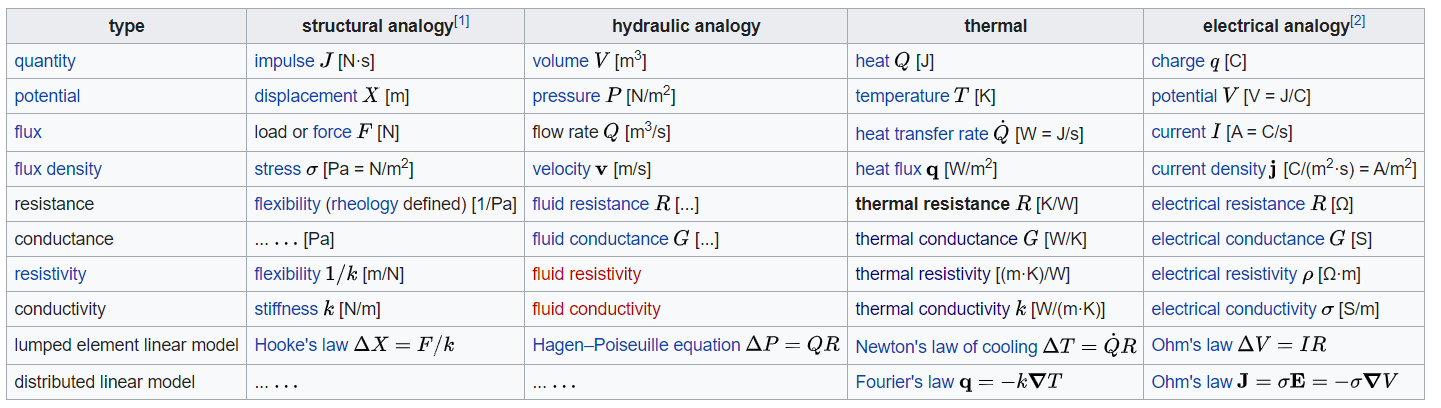
\includegraphics[width=1.0\columnwidth]{Pictures/Analogies.png}
	\caption[Short title]{Analogies table  \cite{AbsTR}}
	\label{fig:Analogies}
	\end{figure} 

The 2R-2C house model structure is implemented as described below. The schematic of an envelope house model has been shown in figure  \ref{fig:envelope2R2C} and the equivalent electrical 2R-2C network with components and topology is given in fig  \ref{fig:elec2R2C}.

\begin{figure}[H]
	\centering
	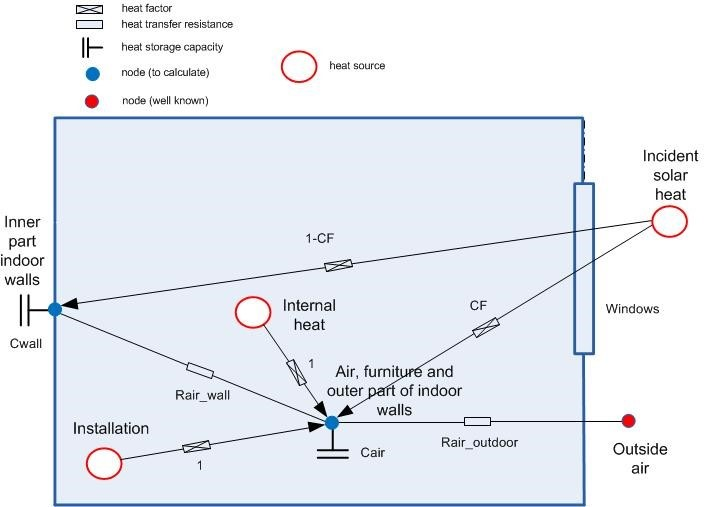
\includegraphics[width=1.0\columnwidth]{Pictures/envelopRC.jpg}
	\caption[Short title]{Schematic of envelope model}
	\label{fig:envelope2R2C}
	\end{figure} 
	

\begin{figure}[H]
	\centering
	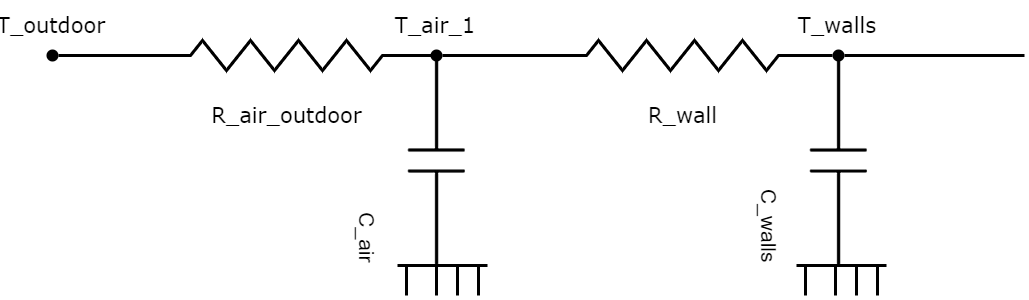
\includegraphics[width=1.0\columnwidth]{Pictures/2R2C_Model.png}
	\caption[Short title]{2R-2C house model}
	\label{fig:elec2R2C}
	\end{figure}
	
The model consists of two capacitances C\textsubscript{air, indoor} and C\textsubscript{wall} and two resistances R\textsubscript{wall} and R\textsubscript{air, outdoor}. The incident solar energy is divided between C\textsubscript{wall} and C\textsubscript{air} through the convection factor CF. It is assumed that both internal heat (lighting, occupancy and electric devices) and supplied heat (installation) initially heat up the indoor air. In fig. \ref{fig:envelope2R2C}, they are fully released at the T\textsubscript{air} node. 

 It is also assumed that furniture and the surface part of the walls have the same temperature as the air and the wall mass is divided between the air and wall mass. Thus, the capacity of the air node consists of the air capacity, furniture capacity and capacity of a part of the walls. \textbf{Appendix A} presents the coefficients in the dwelling model. In the resistance R\textsubscript{air, outdoor} the influence of heat transmission through the outdoor walls and natural ventilation is considered. 
 
For the air and wall nodes the following energy balances can be set up: 

\begin{equation}
C_{air}\frac{dT_{air}}{dt}=\frac{T_{outdoor}-T_{air}}{R_{air_{\_}outdoor}} + \frac{T_{wall}-T_{air}}{R_{air_{\_}wall}} + \dot{Q}_{inst} + \dot{Q}_{internal} + CF\cdot\dot{Q}_{solar}
\end{equation}

\begin{equation}
C_{wall}\frac{dT_{wall}}{dt}=\frac{T_{air}-T_{wall}}{R_{air_{\_}wall}} + (1-CF)\cdot\dot{Q}_{solar}
\end{equation}

 \begin{itemize}
      \item CF: convection factor (solar radiation): the convection factor is the part of the solar radiation that enters the room and is released directly convectively into the room.
      \item $\dot{Q}_{inst}$: delivered heat from heating system (radiator) [W].
      \item $\dot{Q}_{inernal}$: internal heat [W].
      \item $\dot{Q}_{solar}$: heat from solar irradiation [W].
      \item $T_{air}$: indoor air temperature $^o$C.
      \item $T_{outdoor}$: outdoor temperature $^o$C.
      \item $T_{wall}$: wall temperature $^o$C.
      \item $R_{air_{\_}wall}$: walls surface resistance [$\frac{K}{W}$].
      \item $R_{air_{\_}outdoor}$: outdoor surface resistance [$\frac{K}{W}$].
      \item $C_{air}$: air thermal capacitance (heat capacity) [$\frac{J}{K}$]\cite{Thermalmass}.
      \item $C_{wall}$: wall thermal capacitance (heat capacity) [$\frac{J}{K}$]\cite{Thermalmass}.
    \end{itemize}

\newpage   

Total heat transfer of solar irradiation through the glass windows. 
\begin{equation}
\dot{Q}_{solar}=g.\sum(A_{glass}.\dot{q}_{solar})
\end{equation}

\begin{itemize}
    \item $\dot{q}_{solar}$: solar radiation on the outdoor walls [$\frac{W}{m^2}$]. 
    \item g: g value of the glass (ZTA in dutch) [0..1]\cite{zontoetreding}
    \item A: glass surface [$m^2$].
\end{itemize}

%7.6.6.1.2 Ramen met niet-verstrooiende beglazing NTA8800
%https://help.dgmr.nl/bink9/zontoetredingsfactor-zta.html
%https://www.joostdevree.nl/shtmls/zta.shtml
%ISSO-Handboek Zonnestraling: 5.5.1 en 5.2


\newpage
